% !TEX TS-program = pdflatex
% !TEX encoding = UTF-8 Unicode

% This is a simple template for a LaTeX document using the "article" class.
% See "book", "report", "letter" for other types of document.

\documentclass[11pt]{article} % use larger type; default would be 10pt

\usepackage[utf8]{inputenc} % set input encoding (not needed with XeLaTeX)

%%% Examples of Article customizations
% These packages are optional, depending whether you want the features they provide.
% See the LaTeX Companion or other references for full information.

%%% PAGE DIMENSIONS
\usepackage{geometry} % to change the page dimensions
\geometry{a4paper} % or letterpaper (US) or a5paper or....
% \geometry{margin=2in} % for example, change the margins to 2 inches all round
% \geometry{landscape} % set up the page for landscape
%   read geometry.pdf for detailed page layout information

\usepackage{graphicx} % support the \includegraphics command and options

% \usepackage[parfill]{parskip} % Activate to begin paragraphs with an empty line rather than an indent

%%% PACKAGES
\usepackage{booktabs} % for much better looking tables
\usepackage{array} % for better arrays (eg matrices) in maths
\usepackage{paralist} % very flexible & customisable lists (eg. enumerate/itemize, etc.)
\usepackage{verbatim} % adds environment for commenting out blocks of text & for better verbatim
\usepackage{subfig} % make it possible to include more than one captioned figure/table in a single float
% These packages are all incorporated in the memoir class to one degree or another...
\usepackage{pdfpages}
\usepackage{amsmath,mathtools,amsfonts}
\usepackage{bm}
\usepackage{listings}\usepackage{color}

\definecolor{mygreen}{rgb}{0,0.6,0}
\definecolor{mygray}{rgb}{0.5,0.5,0.5}
\definecolor{mymauve}{rgb}{0.58,0,0.82}

\lstset{ 
	backgroundcolor=\color{white},   % choose the background color; you must add \usepackage{color} or \usepackage{xcolor}; should come as last argument
	basicstyle=\footnotesize,        % the size of the fonts that are used for the code
	breakatwhitespace=false,         % sets if automatic breaks should only happen at whitespace
	breaklines=true,                 % sets automatic line breaking
	captionpos=b,                    % sets the caption-position to bottom
	commentstyle=\color{mygreen},    % comment style
	deletekeywords={...},            % if you want to delete keywords from the given language
	escapeinside={\%*}{*)},          % if you want to add LaTeX within your code
	extendedchars=true,              % lets you use non-ASCII characters; for 8-bits encodings only, does not work with UTF-8
	firstnumber=001,                % start line enumeration with line 1000
	frame=single,	                   % adds a frame around the code
	keepspaces=true,                 % keeps spaces in text, useful for keeping indentation of code (possibly needs columns=flexible)
	keywordstyle=\color{blue},       % keyword style
	language=Octave,                 % the language of the code
	morekeywords={*,...},            % if you want to add more keywords to the set
	numbers=left,                    % where to put the line-numbers; possible values are (none, left, right)
	numbersep=5pt,                   % how far the line-numbers are from the code
	numberstyle=\tiny\color{mygray}, % the style that is used for the line-numbers
	rulecolor=\color{black},         % if not set, the frame-color may be changed on line-breaks within not-black text (e.g. comments (green here))
	showspaces=false,                % show spaces everywhere adding particular underscores; it overrides 'showstringspaces'
	showstringspaces=false,          % underline spaces within strings only
	showtabs=false,                  % show tabs within strings adding particular underscores
	stepnumber=2,                    % the step between two line-numbers. If it's 1, each line will be numbered
	stringstyle=\color{mymauve},     % string literal style
	tabsize=2,	                   % sets default tabsize to 2 spaces
	title=\lstname                   % show the filename of files included with \lstinputlisting; also try caption instead of title
}

%%% HEADERS & FOOTERS
\usepackage{fancyhdr} % This should be set AFTER setting up the page geometry
\pagestyle{fancy} % options: empty , plain , fancy
\renewcommand{\headrulewidth}{1pt} % customise the layout...
\lhead{Jesse Sheehan (53366509)}\chead{}\rhead{Will Cowper (81163265)}
\lfoot{}\cfoot{\thepage}\rfoot{}

%%% SECTION TITLE APPEARANCE
%\usepackage{sectsty}
%\allsectionsfont{\sffamily\mdseries\upshape} % (See the fntguide.pdf for font help)
% (This matches ConTeXt defaults)

%%% END Article customizations
\makeatletter
\renewcommand*\env@matrix[1][*\c@MaxMatrixCols c]{%
  \hskip -\arraycolsep
  \let\@ifnextchar\new@ifnextchar
  \array{#1}}
\makeatother

\newenvironment{sysmatrix}[1]
 {\left(\begin{array}{@{}#1@{}}}
 {\end{array}\right)}
\newcommand{\ro}[1]{%
  \xrightarrow{\mathmakebox[\rowidth]{#1}}%
}
\newlength{\rowidth}% row operation width
\AtBeginDocument{\setlength{\rowidth}{3em}}

\title{COSC364 RIPv2 Assignment}
\date{\today}
\author{Jesse Sheehan (53366509)\\ Will Cowper (81163265)}

\begin{document}

\maketitle

\tableofcontents

\newpage

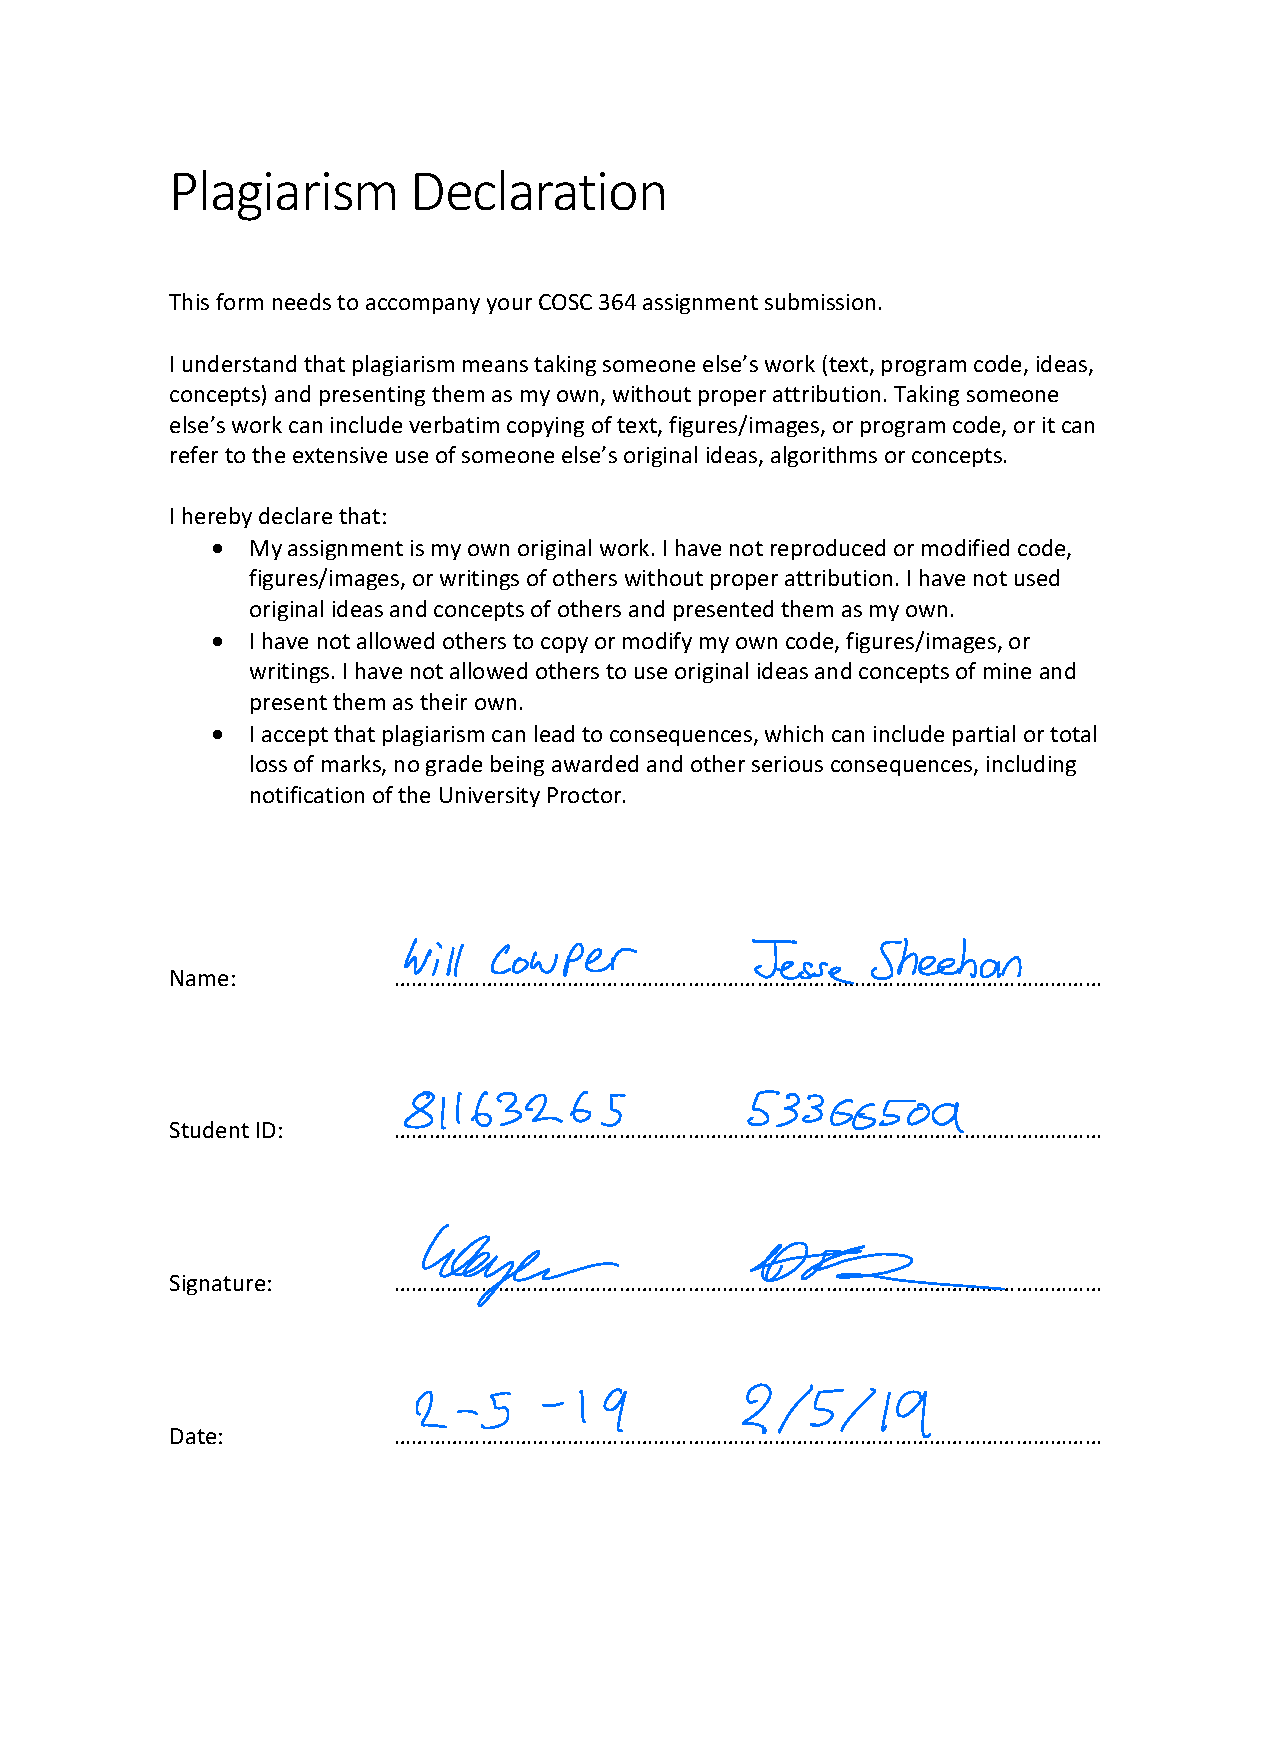
\includepdf[pages=1]{includes/plagiarism.pdf}

\section{Questions}

As required, the following questions have been answered:

\subsection{Contribution}
The contribution toward the entire project was an even split. Both partners felt as though the work they had contributed was worth 50\% each.

\subsection{Reflection}
% Which aspects of your overall program do you consider to be particularly well done?


% Which aspects of your overall program could be improved?

\subsection{Event Processing}
% How have you ensured the atomicity of event processing?
In order to ensure that atomicity of events in our program we have made use of queues and ...


\subsection{Testing}
How have we tested the program?

\newpage
\section{Appendices}

\subsection{Source Code}

\subsubsection{src/\_\_main\_\_.py}
\lstinputlisting[language=Python]{../src/__main__.py}

\subsubsection{src/bencode.py}
\lstinputlisting[language=Python]{../src/bencode.py}

\subsubsection{src/config.py}
\lstinputlisting[language=Python]{../src/config.py}

\subsubsection{src/protocol.py}
\lstinputlisting[language=Python]{../src/protocol.py}

\subsubsection{src/routing\_table\_entry.py}
\lstinputlisting[language=Python]{../src/routing_table_entry.py}

\subsubsection{src/routing\_table.py}
\lstinputlisting[language=Python]{../src/routing_table.py}

\subsubsection{src/server.py}
\lstinputlisting[language=Python]{../src/server.py}

\subsubsection{src/timer.py}
\lstinputlisting[language=Python]{../src/timer.py}

\subsubsection{src/utils.py}
\lstinputlisting[language=Python]{../src/utils.py}

\newpage
\subsection{Configuration Files}

\subsubsection{configs/networks/figure1/1.conf}
\lstinputlisting{../configs/networks/figure1/1.conf}

\subsubsection{configs/networks/figure1/2.conf}
\lstinputlisting{../configs/networks/figure1/2.conf}

\subsubsection{configs/networks/figure1/3.conf}
\lstinputlisting{../configs/networks/figure1/3.conf}

\subsubsection{configs/networks/figure1/4.conf}
\lstinputlisting{../configs/networks/figure1/4.conf}

\subsubsection{configs/networks/figure1/5.conf}
\lstinputlisting{../configs/networks/figure1/5.conf}

\subsubsection{configs/networks/figure1/6.conf}
\lstinputlisting{../configs/networks/figure1/6.conf}

\subsubsection{configs/networks/figure1/7.conf}
\lstinputlisting{../configs/networks/figure1/7.conf}

\newpage
\subsection{Other Files}

\subsubsection{tools/generate\_network.py}
The following file will interactively prompt the user for information about a network. It will then create all the necessary configuration files for the network to run.
\lstinputlisting[language=Python]{../tools/generate_network.py}

\end{document}
